\section{Einleitung}
GEDANKEN:\\
hier vllt mehr auf die Versuche konzentrieren\\
das eher wie einen Praktikumsbericht auslegen\\
kurz und knackig Einführung zu gehen, Pendeltheorie und Analyse durch inverse Kinematik beleuchten\\
Ziel ist die Ermittlung dieser Daten und eine Machbarkeitsstudie zu den Techniken.\\
Die Ergebnisse werden ausgewertet, um zu zeigen, welche Schlüsse aus Belastbaren Daten zu ziehen wären.\\
Der bipedale Gang des Menschen ist ein Erkennungsmerkmal seiner Fortbewegung und weist ein Alleinstellungsmerkmal gegenüber anderen bipedalen Bewegungsstilen auf: die fast vollständige Streckung der Beine (\cite{alexander1992simple}). Die Erforschung der menschlichen Fortbewegung erstreckt sich dabei von der Ganganalyse (alexander und wer noch so alles) über klinische Forschung \autocite{wren2011efficacy} bis hin zur Untersuchung von Laufmustern für Roboter (TLOK-XXX und ...noch eins..).
Ein Schrittzyklus wird grundlegend unterteilt in Standphase und Schwungphase sowie weitere Sub-Phasen, die in Abbildung \ref{fig:Skizze_Phasen} dargestellt sind \autocite{perry1992gait}.
\begin{figure}[h!]
	\centering
	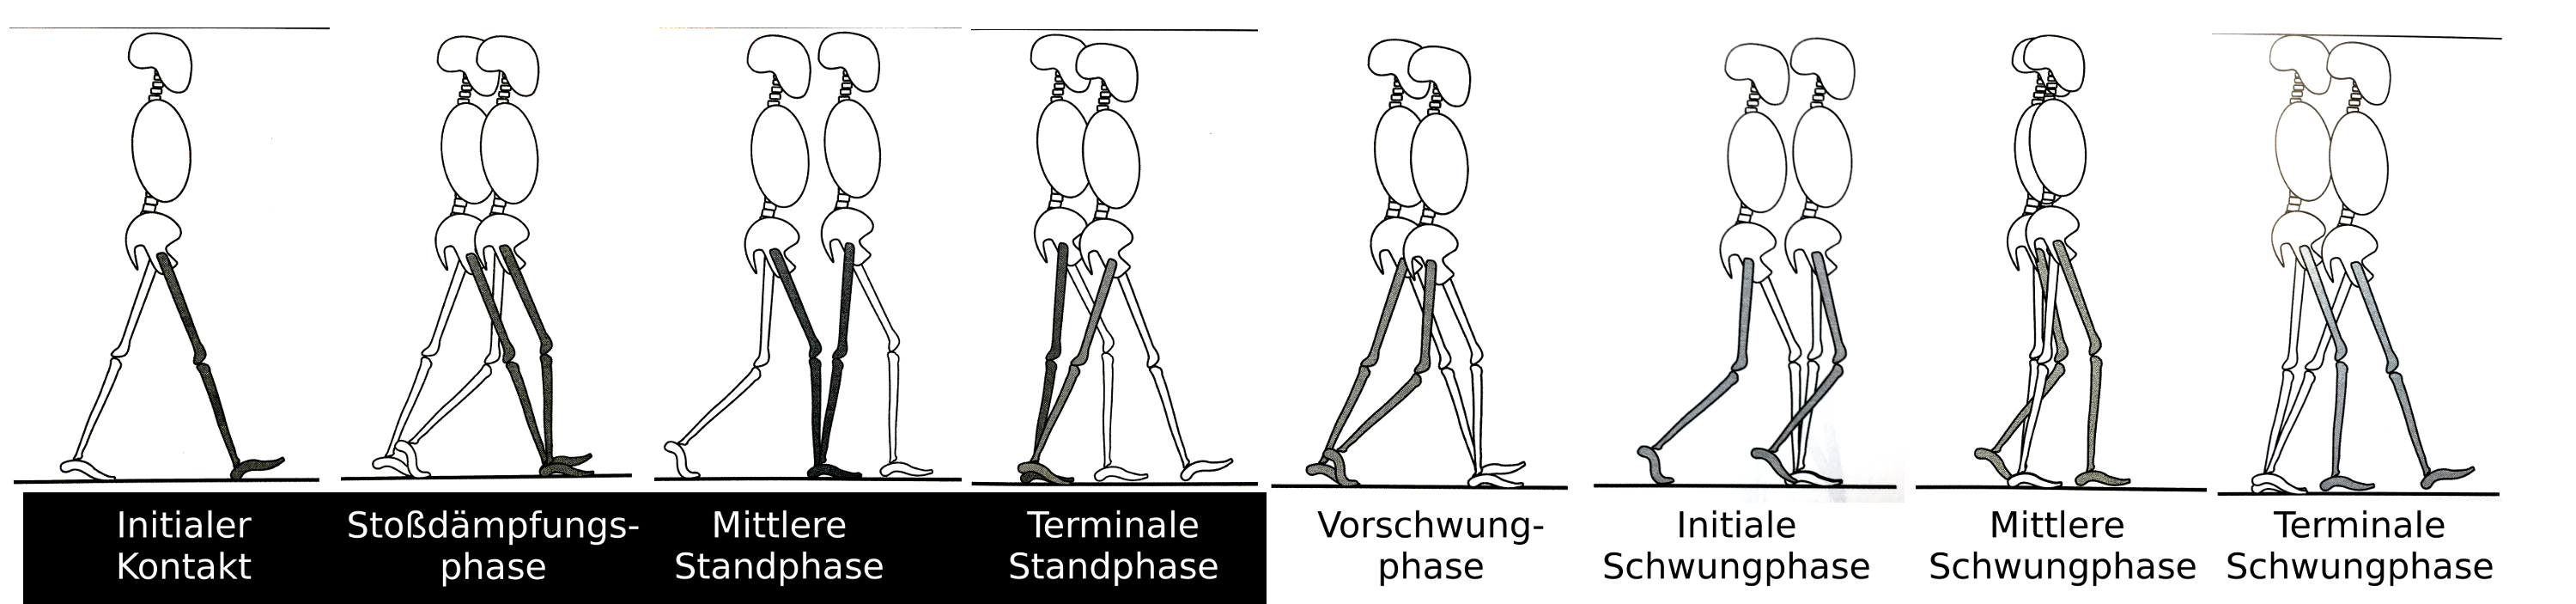
\includegraphics[width=\linewidth]{bilder/Einleitung/Skizze_Gangphasen_small}
	\caption[Gangphasen]{Schrittphasen blablabla. Veränderte Abbildung nach \autocite{perry1992gait}}
	\label{fig:Skizze_Phasen}
\end{figure}

\begin{wrapfigure}{r}{5cm}
	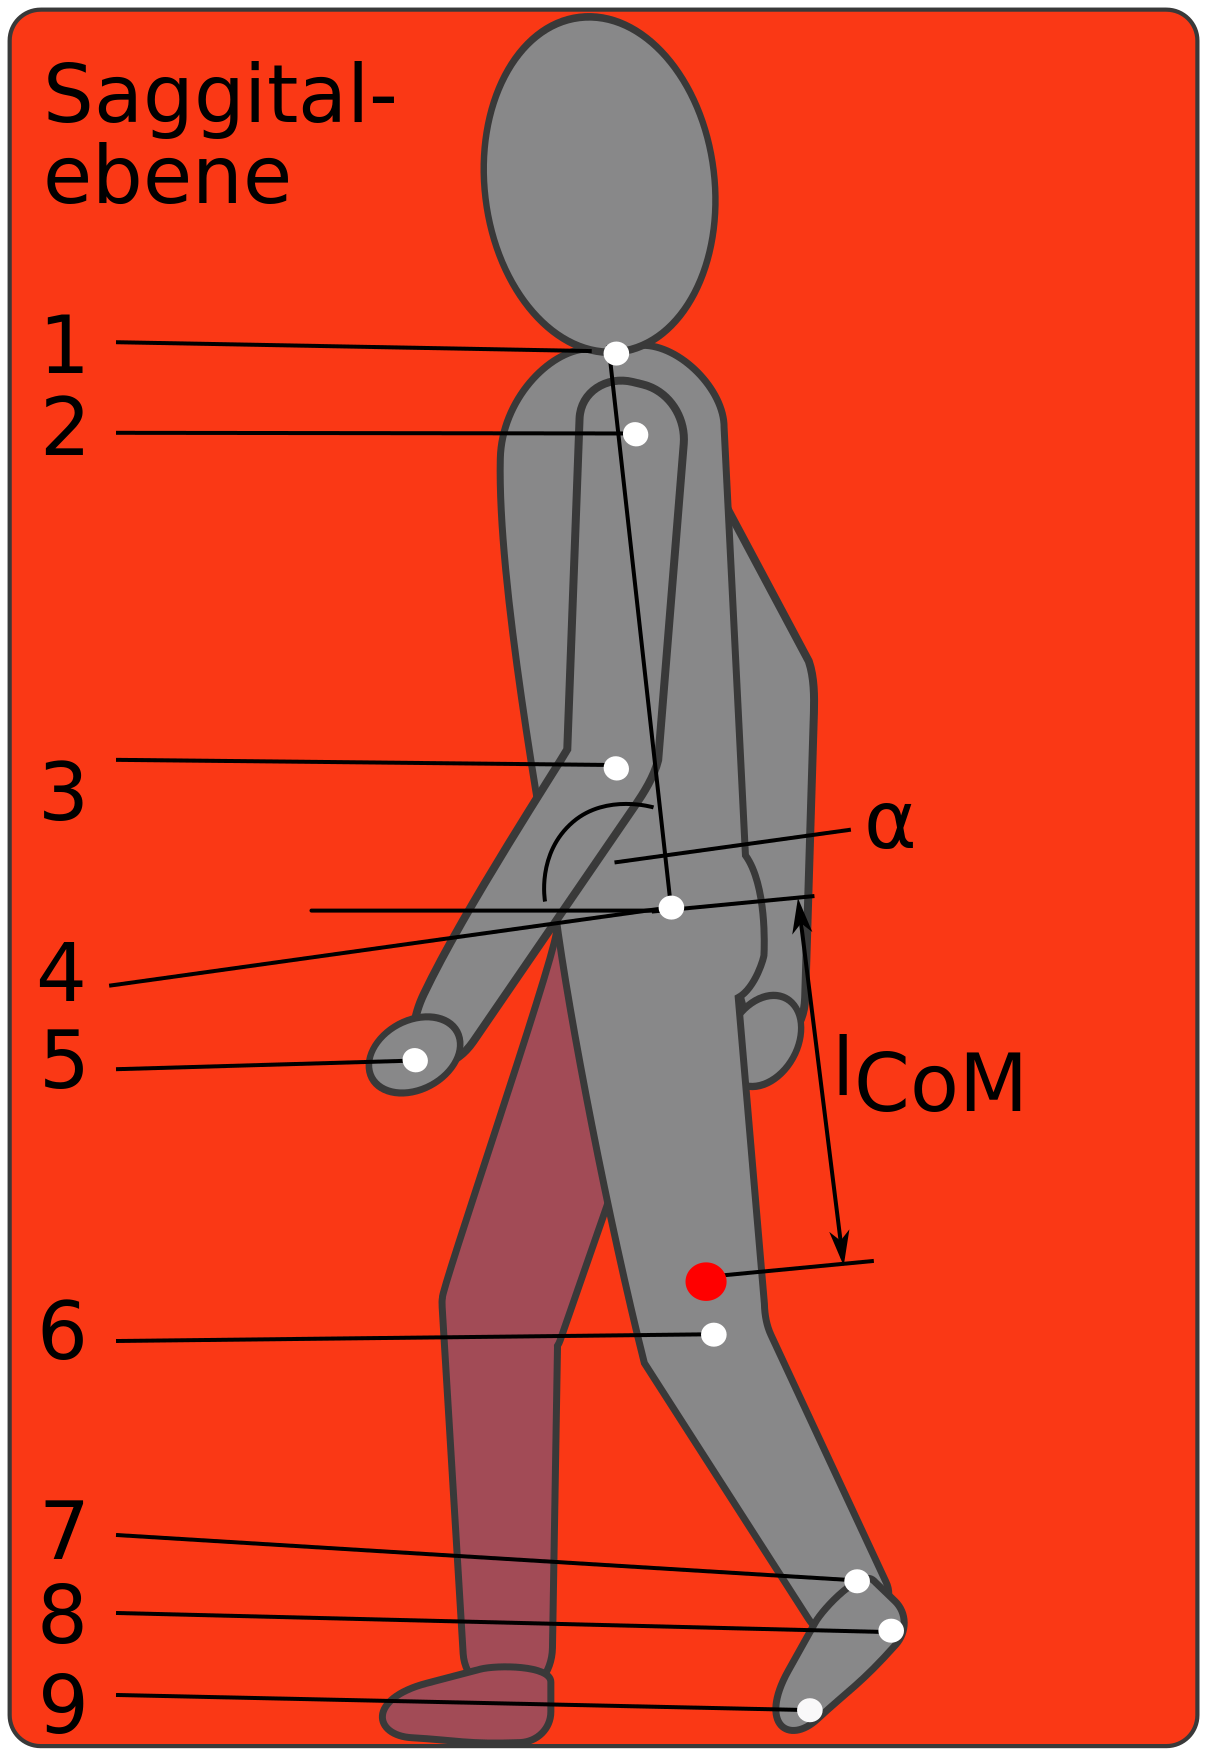
\includegraphics[width=\linewidth]{bilder/Einleitung/Proband_Pendel}
	\caption[Inverses Pendel und untersuchte Gelenke]{Skizze des Probanden in der Sagittalebene mit 9 Markern für: Nacken~-~1, Schulter~-~2, Ellenbogen~-~3, Hüfte~-4, Handgelenk~-~5, Knie~-~6, Knöchel~-~7, Ferse~-~8 und Ballen~9. Massenschwerpunkt des Beines (roter Kreis) und Länge des virtuellen Pendels ($l_{CoM}$) sowie Neigungswinkel des Oberkörpers zur Senkrechten ($\alpha$)}
	\label{fig:Proband_Pendel}
\end{wrapfigure}
Der menschliche Gang lässt sich dabei sehr gut mit dem Modell eines inversen Pendels abstrahieren. Durch das fast vollständig gestreckte Standbein rotiert die Hüfte um den Kontakt-punkt mit dem Boden. Das Schwungbein verhält sich wie ein Pendel und schwingt um die Hüfte. Mit der Distanz des Beinschwerpunktes bis zur Hüfte lässt sich das Bein als mathematisches Pendel abstrahieren und so die Eigenfrequenz des Beines bestimmen. Bewegt man sich mit der Geschwindigkeit fort, bei der das jeweilige Schwungbein mit dieser Periodendauer schwingt, ist für die Beinbewegung keinerlei Energie notwendig (KUO 2007, HIER VLLT ANDERE QUELLE?!?!).\\
Das Modell des inversen Pendels kann durch den subjektiven Energieaufwand beim Gehen überprüft werden. Bewegt man sich mit der Geschwindigkeit fort, bei der die Periodendauer des Schwungbeins der des Pendels entspricht, sollte das Laufen als sehr angenehm empfunden werden und ohne großen Kraftaufwand möglich sein.\\
Weitere Aussagen über den Gang lassen sich durch das Messen der Bodenreaktionskräfte (BRK) treffen. Verbindet man diese mit der im Vorherigen beschriebenen kinematischen Analyse können Momente sowie Lastaufnahme in Y-Richtung sowie ein Abbremsen und Abstoßen in X-Richtung beobachtet werden. 
HIER NOCH WAS ZU DEN ZWEI EXPERIMENTEN!\\
Die sich ergebenden wissenschaftlichen Untersuchungen aus der kinematischen und kinetischen Analyse des menschlichen Ganges sind, wie oben beschrieben, sehr umfassend. In dieser Arbeit wird daher eine qualitative Bewertung des menschlichen Ganges angestrebt. Zunächst soll das Modell des inversen Pendels angewandt werden und der empfundene Laufaufwand mit der Periodendauer des Schwungbeines verglichen werden. Anschließend werden Laufband- und Laufstreckenexperiment auf Unterschiede in der Neigung der Körperachse und der Handtrajektorien veglichen. Hieraus lassen sich Rückschlüsse auf Anpassungen des Ganges an tatsächliche Fortbewegung ziehen (DAS GUT FÜR DIE MEDIZINSICHE UNTERSUCHUNGEN OBEN!!, WÜRDE NOTWENDIGKEITE DER LAUFSTRECKE IN DER BEWEGUNGSANALYSE HERLIETEN).\\
Zusammen mit den Kraftmessungen werden mittels inverser Kinematik auf der Laufstrecke die auftretenden Kräfte und Momente in Knöchel, Knie und Hüfte untersucht und hier Aussagen zu ( JA ZU WAS DENN?? LAUFROBOTER??, BESSERE SCHUHE??) abgeleitet. Alle ermittelten Daten werden mit der Literatur verglichen und die Experimente auf ihre Belastbarkeit geprüft, da auf eine statistische Belastbarkeit der Messdaten verzichtet wurde, um den Umfang der Untersuchungen zu erhöhen.\\
HIER AUF INVERSES UND SCHWERKRAFTPENDEL EINGEHEN!!\\

Die inverse Dynamik erlaubt die Bestimmung von Kraft und Momenten in Gelenken, ohne Messungen an den jeweiligen Gelenken durchführen zu müssen.